\documentclass{article}
\usepackage{amsmath}
\usepackage{graphicx}

\begin{document}

\title{Calcul du Facteur \( a \) pour Différentes Bandes de Fréquence}
\author{}
\date{}
\maketitle

\section{Introduction}
Pour maximiser la réflectivité, nous devons choisir une géométrie de cristal qui possède un gap de bande photonique tout en restant réalisable sur le plan pratique. Dans cet exemple conceptuel bidimensionnel, nous étudions une structure woodpile réalisée en Macor, un matériau diélectrique céramique avec une permittivité relative \( \epsilon_r = 5.64 \). Cette géométrie présente de grands gaps de bande pour les modes TM, ce qui en fait une option intéressante pour des applications photoniques.

\section{Théorie}
La longueur d'onde \( \lambda \) est liée à la fréquence \( f \) par la relation :
\[
\lambda = \frac{c}{f}
\]
où \( c \) est la vitesse de la lumière dans le vide (\( c = 299\,792\,458 \) m/s).

La constante du réseau \( a \) est alors donnée par :
\[
a = \lambda \times \text{fréquence normalisée}
\]
Dans notre cas, la fréquence normalisée est de 0.6694.

\section{Calculs}
Nous allons calculer \( a \) pour les bandes de fréquence suivantes : X-Band, Ku-Band, K-Band, et Ka-Band.

\subsection{X-Band (8.2–12.4 GHz)}
Pour \( f_{\text{min}} = 8.2 \times 10^9 \) Hz :
\[
\lambda_{\text{min}} = \frac{299\,792\,458}{8.2 \times 10^9} = 3.656 \times 10^{-2} \text{ m}
\]
\[
a_{\text{min}} = 3.656 \times 10^{-2} \times 0.6694 = 2.447 \times 10^{-2} \text{ m}
\]

Pour \( f_{\text{milieu}} = 10.3 \times 10^9 \) Hz :
\[
\lambda_{\text{milieu}} = \frac{299\,792\,458}{10.3 \times 10^9} = 2.91 \times 10^{-2} \text{ m}
\]
\[
a_{\text{milieu}} = 2.91 \times 10^{-2} \times 0.6694 = 1.948 \times 10^{-2} \text{ m}
\]

Pour \( f_{\text{max}} = 12.4 \times 10^9 \) Hz :
\[
\lambda_{\text{max}} = \frac{299\,792\,458}{12.4 \times 10^9} = 2.417 \times 10^{-2} \text{ m}
\]
\[
a_{\text{max}} = 2.417 \times 10^{-2} \times 0.6694 = 1.618 \times 10^{-2} \text{ m}
\]

\subsection{Ku-Band (12.4–18 GHz)}
Pour \( f_{\text{min}} = 12.4 \times 10^9 \) Hz :
\[
\lambda_{\text{min}} = 2.417 \times 10^{-2} \text{ m}
\]
\[
a_{\text{min}} = 2.417 \times 10^{-2} \times 0.6694 = 1.618 \times 10^{-2} \text{ m}
\]

Pour \( f_{\text{milieu}} = 15.2 \times 10^9 \) Hz :
\[
\lambda_{\text{milieu}} = \frac{299\,792\,458}{15.2 \times 10^9} = 1.97 \times 10^{-2} \text{ m}
\]
\[
a_{\text{milieu}} = 1.97 \times 10^{-2} \times 0.6694 = 1.319 \times 10^{-2} \text{ m}
\]

Pour \( f_{\text{max}} = 18 \times 10^9 \) Hz :
\[
\lambda_{\text{max}} = \frac{299\,792\,458}{18 \times 10^9} = 1.666 \times 10^{-2} \text{ m}
\]
\[
a_{\text{max}} = 1.666 \times 10^{-2} \times 0.6694 = 1.115 \times 10^{-2} \text{ m}
\]

\subsection{K-Band (18–26.5 GHz)}
Pour \( f_{\text{min}} = 18 \times 10^9 \) Hz :
\[
\lambda_{\text{min}} = 1.666 \times 10^{-2} \text{ m}
\]
\[
a_{\text{min}} = 1.666 \times 10^{-2} \times 0.6694 = 1.115 \times 10^{-2} \text{ m}
\]

Pour \( f_{\text{milieu}} = 22.25 \times 10^9 \) Hz :
\[
\lambda_{\text{milieu}} = \frac{299\,792\,458}{22.25 \times 10^9} = 1.35 \times 10^{-2} \text{ m}
\]
\[
a_{\text{milieu}} = 1.35 \times 10^{-2} \times 0.6694 = 9.03 \times 10^{-3} \text{ m}
\]

Pour \( f_{\text{max}} = 26.5 \times 10^9 \) Hz :
\[
\lambda_{\text{max}} = \frac{299\,792\,458}{26.5 \times 10^9} = 1.131 \times 10^{-2} \text{ m}
\]
\[
a_{\text{max}} = 1.131 \times 10^{-2} \times 0.6694 = 7.569 \times 10^{-3} \text{ m}
\]

\subsection{Ka-Band (26.5–40 GHz)}
Pour \( f_{\text{min}} = 26.5 \times 10^9 \) Hz :
\[
\lambda_{\text{min}} = 1.131 \times 10^{-2} \text{ m}
\]
\[
a_{\text{min}} = 1.131 \times 10^{-2} \times 0.6694 = 7.569 \times 10^{-3} \text{ m}
\]

Pour \( f_{\text{milieu}} = 33.25 \times 10^9 \) Hz :
\[
\lambda_{\text{milieu}} = \frac{299\,792\,458}{33.25 \times 10^9} = 9.01 \times 10^{-3} \text{ m}
\]
\[
a_{\text{milieu}} = 9.01 \times 10^{-3} \times 0.6694 = 6.03 \times 10^{-3} \text{ m}
\]

Pour \( f_{\text{max}} = 40 \times 10^9 \) Hz :
\[
\lambda_{\text{max}} = \frac{299\,792\,458}{40 \times 10^9} = 7.495 \times 10^{-3} \text{ m}
\]
\[
a_{\text{max}} = 7.495 \times 10^{-3} \times 0.6694 = 5.017 \times 10^{-3} \text{ m}
\]
\section{Schéma Technique}
\begin{figure}[h!]
    \centering
    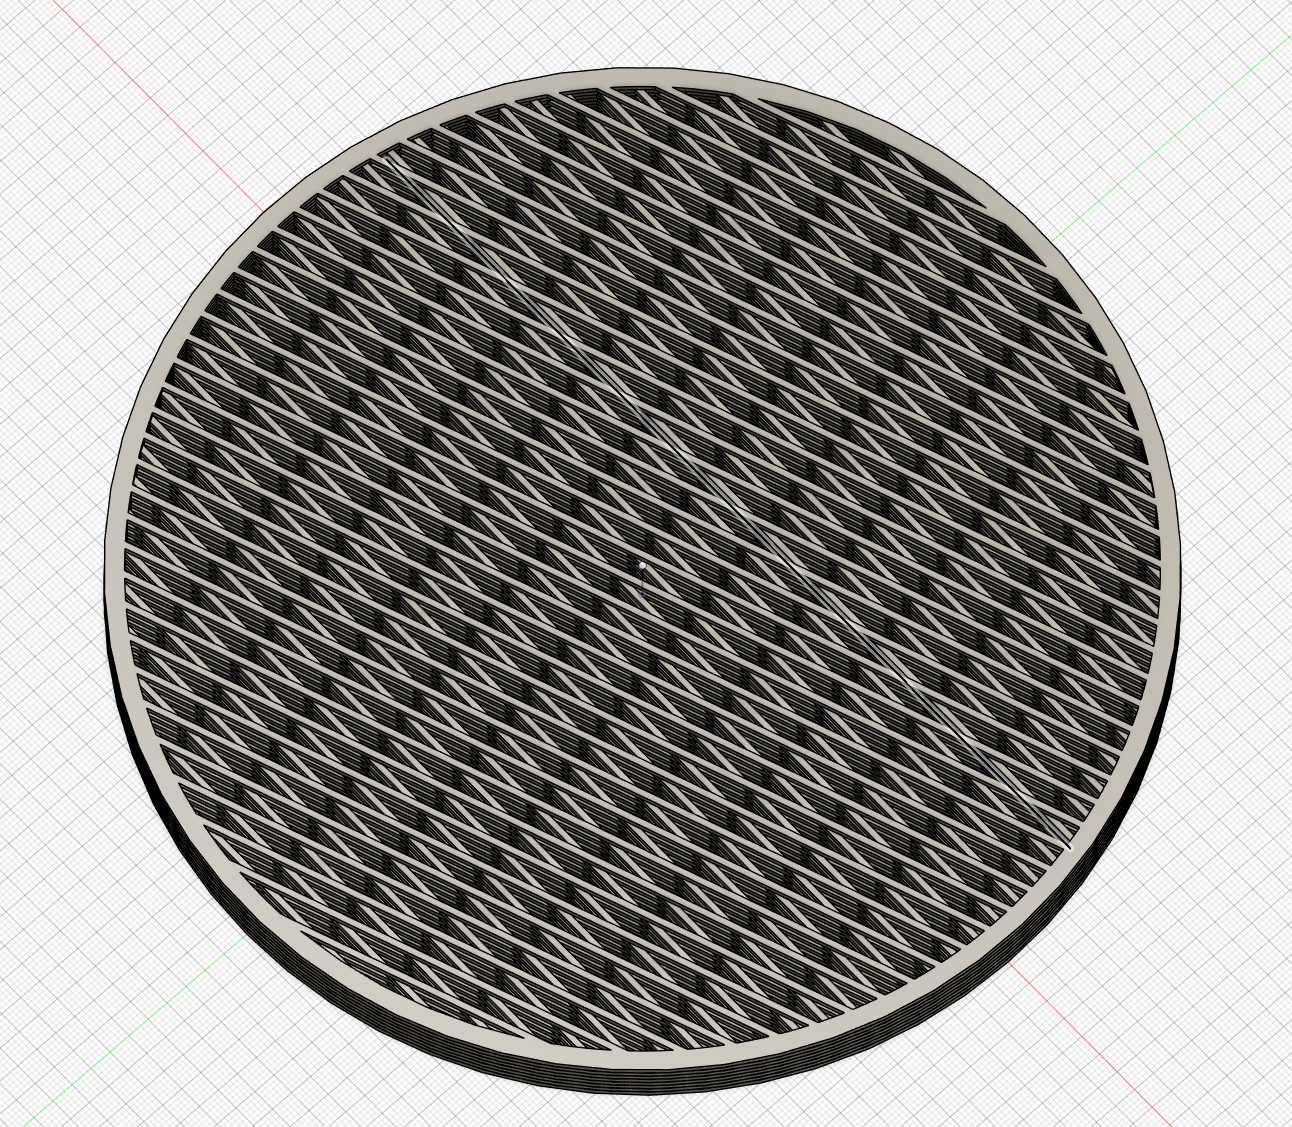
\includegraphics[width=0.8\textwidth]{Images/CaM9WdelYQNDJb8v.png}
    \caption{Schéma technique de la structure woodpile.}
    \label{fig:schema}
\end{figure}

\begin{itemize}
    \item \textbf{Constante de réseau} :  
    \[
    a
    \]
    \item \textbf{Hauteur des tiges} :  
    \[
    \text{rods\_height} = 0.3 \cdot a
    \]
    \item \textbf{Décalage des tiges} :  
    \[
    \text{rods\_shift} = 0.25 \cdot a
    \]
    \item \textbf{Largeur des tiges} :  
    \[
    \text{rods\_w} = 0.25 \cdot a
    \]
    
\end{itemize}


\section{Dimensions à Usiner}
Pour une plaque de 15 cm x 15 cm, nous pouvons calculer le nombre de cellules unités que nous pouvons placer en fonction de la constante du réseau \( a \).

La surface de la plaque est donnée par :
\[
\text{Surface} = 0.15 \, \text{m} \times 0.15 \, \text{m} = 0.0225 \, \text{m}^2
\]

Le nombre de cellules unités que nous pouvons placer est calculé en divisant la surface de la plaque par la surface d'une cellule unité (qui est \( a^2 \)).

\subsection{X-Band (8.2–12.4 GHz)}
\begin{itemize}
    \item Pour \( a_{\text{min}} = 2.447 \times 10^{-2} \) m :
    \[
    \text{Surface d'une cellule} = (2.447 \times 10^{-2})^2 = 5.986 \times 10^{-4} \, \text{m}^2
    \]
    \[
    \text{Nombre de cellules} = \frac{0.0225}{5.986 \times 10^{-4}} \approx 37
    \]

    \item Pour \( a_{\text{milieu}} = 1.948 \times 10^{-2} \) m :
    \[
    \text{Surface d'une cellule} = (1.948 \times 10^{-2})^2 = 3.793 \times 10^{-4} \, \text{m}^2
    \]
    \[
    \text{Nombre de cellules} = \frac{0.0225}{3.793 \times 10^{-4}} \approx 59
    \]

    \item Pour \( a_{\text{max}} = 1.618 \times 10^{-2} \) m :
    \[
    \text{Surface d'une cellule} = (1.618 \times 10^{-2})^2 = 2.617 \times 10^{-4} \, \text{m}^2
    \]
    \[
    \text{Nombre de cellules} = \frac{0.0225}{2.617 \times 10^{-4}} \approx 86
    \]
\end{itemize}

\subsection{Ku-Band (12.4–18 GHz)}
\begin{itemize}
    \item Pour \( a_{\text{min}} = 1.618 \times 10^{-2} \) m :
    \[
    \text{Surface d'une cellule} = (1.618 \times 10^{-2})^2 = 2.617 \times 10^{-4} \, \text{m}^2
    \]
    \[
    \text{Nombre de cellules} = \frac{0.0225}{2.617 \times 10^{-4}} \approx 86
    \]

    \item Pour \( a_{\text{milieu}} = 1.319 \times 10^{-2} \) m :
    \[
    \text{Surface d'une cellule} = (1.319 \times 10^{-2})^2 = 1.739 \times 10^{-4} \, \text{m}^2
    \]
    \[
    \text{Nombre de cellules} = \frac{0.0225}{1.739 \times 10^{-4}} \approx 129
    \]

    \item Pour \( a_{\text{max}} = 1.115 \times 10^{-2} \) m :
    \[
    \text{Surface d'une cellule} = (1.115 \times 10^{-2})^2 = 1.243 \times 10^{-4} \, \text{m}^2
    \]
    \[
    \text{Nombre de cellules} = \frac{0.0225}{1.243 \times 10^{-4}} \approx 181
    \]
\end{itemize}

\subsection{K-Band (18–26.5 GHz)}
\begin{itemize}
    \item Pour \( a_{\text{min}} = 1.115 \times 10^{-2} \) m :
    \[
    \text{Surface d'une cellule} = (1.115 \times 10^{-2})^2 = 1.243 \times 10^{-4} \, \text{m}^2
    \]
    \[
    \text{Nombre de cellules} = \frac{0.0225}{1.243 \times 10^{-4}} \approx 181
    \]

    \item Pour \( a_{\text{milieu}} = 9.03 \times 10^{-3} \) m :
    \[
    \text{Surface d'une cellule} = (9.03 \times 10^{-3})^2 = 8.154 \times 10^{-5} \, \text{m}^2
    \]
    \[
    \text{Nombre de cellules} = \frac{0.0225}{8.154 \times 10^{-5}} \approx 276
    \]

    \item Pour \( a_{\text{max}} = 7.569 \times 10^{-3} \) m :
    \[
    \text{Surface d'une cellule} = (7.569 \times 10^{-3})^2 = 5.728 \times 10^{-5} \, \text{m}^2
    \]
    \[
    \text{Nombre de cellules} = \frac{0.0225}{5.728 \times 10^{-5}} \approx 393
    \]
\end{itemize}

\subsection{Ka-Band (26.5–40 GHz)}
\begin{itemize}
    \item Pour \( a_{\text{min}} = 7.569 \times 10^{-3} \) m :
    \[
    \text{Surface d'une cellule} = (7.569 \times 10^{-3})^2 = 5.728 \times 10^{-5} \, \text{m}^2
    \]
    \[
    \text{Nombre de cellules} = \frac{0.0225}{5.728 \times 10^{-5}} \approx 393
    \]

    \item Pour \( a_{\text{milieu}} = 6.03 \times 10^{-3} \) m :
    \[
    \text{Surface d'une cellule} = (6.03 \times 10^{-3})^2 = 3.636 \times 10^{-5} \, \text{m}^2
    \]
    \[
    \text{Nombre de cellules} = \frac{0.0225}{3.636 \times 10^{-5}} \approx 619
    \]

    \item Pour \( a_{\text{max}} = 5.017 \times 10^{-3} \) m :
    \[
    \text{Surface d'une cellule} = (5.017 \times 10^{-3})^2 = 2.517 \times 10^{-5} \, \text{m}^2
    \]
    \[
    \text{Nombre de cellules} = \frac{0.0225}{2.517 \times 10^{-5}} \approx 894
    \]
\end{itemize}


\section{Conclusion}
En résumé, les valeurs de la constante du réseau \( a \) pour les différentes bandes de fréquence et le nombre de cellules unités que nous pouvons placer dans une plaque de 15 cm x 15 cm sont les suivants :

\begin{itemize}
    \item \textbf{X-Band (8.2–12.4 GHz)} :
    \begin{itemize}
        \item \( a_{\text{min}} = 2.447 \times 10^{-2} \) m : 37 cellules
        \item \( a_{\text{milieu}} = 1.948 \times 10^{-2} \) m : 59 cellules
        \item \( a_{\text{max}} = 1.618 \times 10^{-2} \) m : 86 cellules
    \end{itemize}
    \item \textbf{Ku-Band (12.4–18 GHz)} :
    \begin{itemize}
        \item \( a_{\text{min}} = 1.618 \times 10^{-2} \) m : 86 cellules
        \item \( a_{\text{milieu}} = 1.319 \times 10^{-2} \) m : 129 cellules
        \item \( a_{\text{max}} = 1.115 \times 10^{-2} \) m : 181 cellules
    \end{itemize}
    \item \textbf{K-Band (18–26.5 GHz)} :
    \begin{itemize}
        \item \( a_{\text{min}} = 1.115 \times 10^{-2} \) m : 181 cellules
        \item \( a_{\text{milieu}} = 9.03 \times 10^{-3} \) m : 276 cellules
        \item \( a_{\text{max}} = 7.569 \times 10^{-3} \) m : 393 cellules
    \end{itemize}
    \item \textbf{Ka-Band (26.5–40 GHz)} :
    \begin{itemize}
        \item \( a_{\text{min}} = 7.569 \times 10^{-3} \) m : 393 cellules
        \item \( a_{\text{milieu}} = 6.03 \times 10^{-3} \) m : 619 cellules
        \item \( a_{\text{max}} = 5.017 \times 10^{-3} \) m : 894 cellules
    \end{itemize}
\end{itemize}

Ces résultats montrent comment la constante du réseau \( a \) change en fonction des différentes bandes de fréquence et comment cela affecte le nombre de cellules unités que nous pouvons placer dans une plaque de 15 cm x 15 cm. Ces informations sont cruciales pour la conception de structures photoniques avec des gaps de bande spécifiques et pour déterminer les dimensions à usiner pour des applications pratiques.
\end{document}